% 附录 T：磁面、磁岛与磁通量管：拓扑如何决定约束（v1.17.0 新增）
% 数值唯一来源：tools/calc/appT_calc.py -> tools/calc/appT_calc.txt（正文与门禁的唯一来源）
% 时间单位写成 s/ms，避免中文字符进入数学字体；全部数字可用仓库脚本复算。
% 版权口径：只借鉴经典教材与文献的物理结论、公式形式与题型；文字、数值与表格自拟并独立复算。
% 离线环境无法核验 DOI，故只给书名、作者、年份、卷期页。
% 本附录与附录 S 共用同一组三个工作点，q 剖面为教学剖面（在正文中声明）。

\section{磁面、安全因子与"拓扑的语言"}
\label{sec:app-t-topology}

附录 S 把约束写成一个数 $\tau_E$，再反推出有效输运系数 $\chi_{\mathrm{eff}}$。但那个数是
\textbf{磁面平均}的结果：它假定热量沿着"一层一层的磁面"往外走。真实磁场一旦被扰动，
磁面本身会被撕开、重联、缠成岛——这时"层"的图景失效，而失效处正是输运最凶的地方。
本附录处理的就是这件事：\textbf{拓扑}。

先把语言定下来。轴对称托卡马克的磁场可以写成

\begin{equation}
\mathbf{B}=\nabla\psi\times\nabla\phi+F\nabla\phi ,
\label{eq:app-t-fluxfunc}
\end{equation}

其中 $\psi$ 是极向磁通函数（$\psi=\text{const}$ 就是磁面），$F=RB_\phi$ 是环向场函数，
$\phi$ 是环向角。把式 \eqref{eq:app-t-fluxfunc} 投影到极向面，得到两条最有用的关系：

\begin{equation}
B_\theta(r)=\frac{B\,r}{q(r)\,R},
\qquad\text{与}\qquad
q(r)=\frac{rB_\phi}{RB_\theta},
\label{eq:app-t-bo}
\end{equation}

这里用了大环径比近似 $B\approx B_\phi$。$q$ 叫安全因子，它的几何含义是
\textbf{磁力线绕环向 $q$ 圈才绕极向一圈}；等价说法是磁力线在一个磁面上的"螺距比"。

\begin{table}[htbp]
  \centering
  \caption{三个工作点的 $q$ 剖面参数。$q_0$ 与 $q_{95}$ 是剖面端点（轴心与 $95\%$ 磁通面）；
    "设计/典型值"取该量级装置的公开运行区间，"本书公式"指第 10 章 10.8 节的
    $q_{95}\approx 5a^2B(1+\kappa^2)/(2RI_p)$。}
  \label{tab:app-t-q95}
  \begin{tabular}{@{}p{3.0cm}p{1.4cm}p{1.9cm}p{1.9cm}p{1.6cm}p{1.5cm}p{1.5cm}@{}}
    \toprule
    装置 & $q_0$ & $q_{95}$ 设计 & $q_{95}$ 本书公式 & 差值 & $a$ [m] & $B$ [T] \\
    \midrule
    D1 ITER 量级 & $1.05$ & $3.00$ & $2.22$ & $+0.78$ & $2.00$ & $5.3$ \\
    D2 JET 量级 & $1.00$ & $3.90$ & $3.91$ & $-0.01$ & $1.25$ & $3.0$ \\
    D3 DIII-D 量级 & $0.85$ & $4.00$ & $3.99$ & $+0.01$ & $0.67$ & $2.1$ \\
    \bottomrule
  \end{tabular}
\end{table}

表 \ref{tab:app-t-q95} 里 D1 那一行的差 $+0.78$ 值得停一下：本书的简化公式
\textbf{系统性低估了强三角变位形的 $q_{95}$}（第 10 章已说明该公式忽略了三角形变与内感，
ITER 官方设计值为 $3.0$，简化式给 $2.2$）。这个差别不是小数点问题——$q_{95}$ 直接决定
有理面（下一节）落在哪里，而 D2、D3 的公式值与典型值几乎重合，说明该公式对
\textbf{低三角变、中等拉长}的装置够用。本附录后面的计算一律用"设计/典型值"一列。

\begin{tip}{磁通量管（flux tube）：把三维问题降成一维}{tip-app-t-flux}
在磁面上取一小块垂直截面，让它的边界由同一族磁力线扫出来，得到的管状体积叫磁通量管。
它的关键性质是\textbf{磁通守恒}：沿管长 $l$，$BA=\text{const}$（$A$ 为截面积）。
于是磁力线越密（$B$ 越大）管子越细，而管内的平行输运几乎不受磁场约束——
这就是下一节"两条路"的几何来源。
\end{tip}

{\footnotesize
\textbf{出处：}Wesson《Tokamaks》第 4 版第 3 章（磁面坐标与 $q$ 的定义）；
Chen《Introduction to Plasma Physics and Controlled Fusion》第 2 版第 4 章
（磁通函数与磁面）；Freidberg《Ideal MHD》（Cambridge，2014）第 10 章
（安全因子与磁力线拓扑）。三个装置的 $q_0$、$q_{95}$ 取自各装置公开运行区间，
"本书公式"一列由仓库脚本按第 10 章公式复算。
}

\begin{figure}[htbp]
\centering
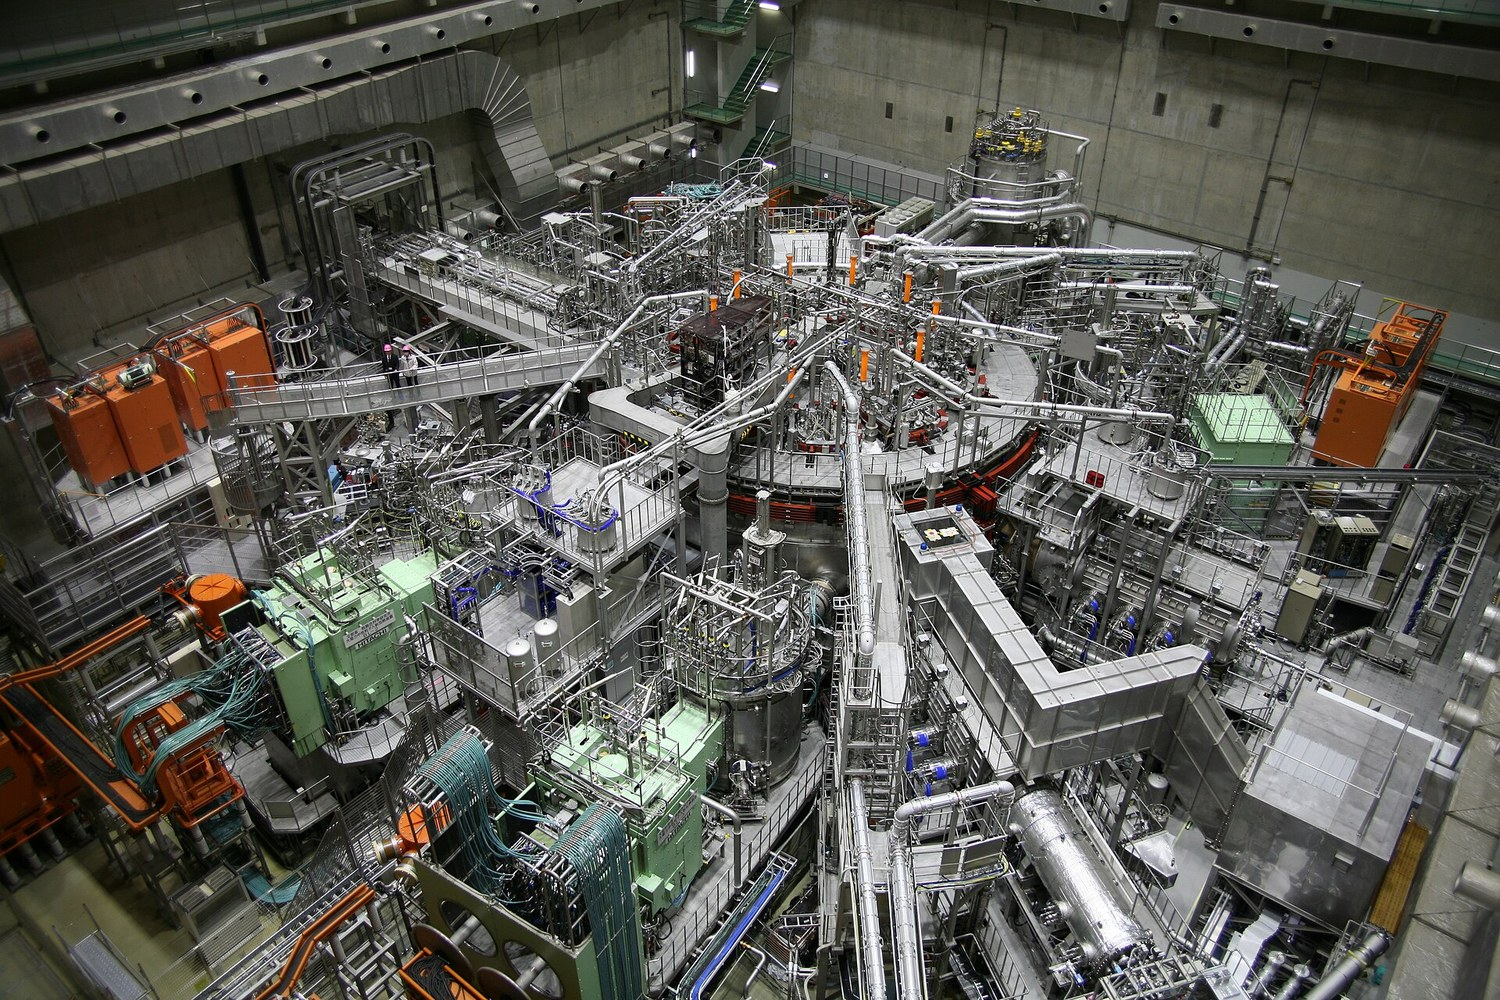
\includegraphics[width=0.72\textwidth]{../figures/t_lhd_heliotron.jpg}
\caption{仿星器不需要等离子体电流：图中这组螺旋线圈直接把旋转变换写进磁场。本节算的 q 剖面与有理面位置，就是这类线圈几何的直接后果。}
\label{fig:photo-appt2}
\figsource{National Institute for Fusion Science (NIFS)，CC BY-SA 4.0（Wikimedia Commons）}
\end{figure}

\section{安全因子剖面与有理面}
\label{sec:app-t-rational}

$q$ 不是一个数，而是一个剖面。为了能算，本附录取一条\textbf{教学剖面}：

\begin{equation}
q(\rho)=q_0+(q_{95}-q_0)\,\rho^2,
\qquad \rho\equiv\frac{r}{a},
\label{eq:app-t-qprofile}
\end{equation}

它在轴上取 $q_0$、在边缘取 $q_{95}$，且 $q$ 随 $r$ 单调上升——真实剖面大体如此（细节由
电流密度剖面决定）。由式 \eqref{eq:app-t-qprofile} 得到局部剪切

\begin{equation}
q'(r)=\frac{\diff q}{\diff r}=\frac{2(q_{95}-q_0)\,r}{a^2},
\qquad
s(r)\equiv\frac{r\,q'}{q},
\label{eq:app-t-shear}
\end{equation}

$s$ 是无量纲量，叫磁剪切：它衡量"相邻磁面上的螺距差多少"。

\textbf{有理面（rational surface）}是满足

\begin{equation}
q(r_{mn})=\frac{m}{n}
\label{eq:app-t-resonance}
\end{equation}

的磁面（$m,n$ 互质整数）。它的特殊性来自平行波数：一个螺旋扰动
$\propto\exp[i(m\theta-n\phi)]$ 在磁面上的平行波数是

\begin{equation}
k_\parallel=\frac{m-nq(r)}{q(r)\,R},
\label{eq:app-t-kpar}
\end{equation}

\textbf{在有理面上 $k_\parallel=0$}。这一条是整个附录的枢纽：平行方向没有波数，
意味着扰动在平行方向"没有恢复力"、也不受平行输运的平滑（下一节会看到平行输运有多强），
于是扰动可以在有理面附近自由地重联磁场、撕开磁面。

\begin{table}[htbp]
  \centering
  \caption{三个装置的有理面位置与局部量（$q$ 剖面取式 \eqref{eq:app-t-qprofile}）。
    $B_\theta$ 由式 \eqref{eq:app-t-bo} 给出，$L_q\equiv q/q'$ 是剪切长度。}
  \label{tab:app-t-surfaces}
  \begin{tabular}{@{}p{3.0cm}p{1.4cm}p{1.5cm}p{1.5cm}p{1.6cm}p{1.6cm}p{1.4cm}p{1.5cm}@{}}
    \toprule
    装置 & $q$ 面 & $\rho$ & $r$ [m] & $B_\theta$ [T] & $q'$ [1/m] & $s$ & $L_q$ [m] \\
    \midrule
    D1 ITER 量级 & $3/2$ & $0.4804$ & $0.9608$ & $0.5475$ & $0.9367$ & $0.6000$ & $1.6013$ \\
    D1 ITER 量级 & $2/1$ & $0.6980$ & $1.3960$ & $0.5967$ & $1.3611$ & $0.9500$ & $1.4694$ \\
    D2 JET 量级 & $3/2$ & $0.4152$ & $0.5190$ & $0.3507$ & $1.9267$ & $0.6667$ & $0.7786$ \\
    D2 JET 量级 & $2/1$ & $0.5872$ & $0.7340$ & $0.3720$ & $2.7247$ & $1.0000$ & $0.7340$ \\
    D3 DIII-D 量级 & $1/1$ & $0.2182$ & $0.1462$ & $0.1839$ & $2.0519$ & $0.3000$ & $0.4874$ \\
    D3 DIII-D 量级 & $3/2$ & $0.4543$ & $0.3044$ & $0.2551$ & $4.2714$ & $0.8667$ & $0.3512$ \\
    D3 DIII-D 量级 & $2/1$ & $0.6042$ & $0.4048$ & $0.2545$ & $5.6815$ & $1.1500$ & $0.3520$ \\
    \bottomrule
  \end{tabular}
\end{table}

表 \ref{tab:app-t-surfaces} 有三个可以直接读出的结论：

\textbf{（1）有理面的半径对 $q_0$ 极敏感。}D1 的 $q_0=1.05>1$，所以\textbf{根本没有 $q=1$ 面}
（无锯齿，见 T.7 节）；D2 的 $q_0=1.00$ 恰好压在 $1$ 上；D3 的 $q_0=0.85$ 才在
$\rho=0.218$ 处留出 $q=1$ 面。轴上 $q_0$ 差 $0.2$，决定了"有没有锯齿"这种定性差别。

\textbf{（2）$B_\theta$ 只有环向场的 $1/10$ 量级。}D1 在 $r=1.4\ \mathrm{m}$ 处
$B_\theta=0.60\ \mathrm{T}$，而 $B=5.3\ \mathrm{T}$。这个比值就是 $r/(qR)$——
它后面会出现在岛宽公式里，也是"扰动磁场只要百分之几就能撕开磁面"的原因。

\textbf{（3）剪切 $s$ 是 $0.3$--$1.2$ 的量级，而且有一个漂亮的恒等式。}对式
\eqref{eq:app-t-qprofile} 这样的剖面，把 $q'$ 代进式 \eqref{eq:app-t-shear} 后
$\rho$ 被消掉：

\begin{equation}
s(r)=2\,\frac{q(r)-q_0}{q(r)}=2-\frac{2q_0}{q(r)} ,
\label{eq:app-t-sidentity}
\end{equation}

\textbf{剪切只由轴上 $q_0$ 与当地 $q$ 决定}。读者可据此核对表
\ref{tab:app-t-surfaces}：D1 在 $q=2$ 面 $s=2-2.10/2=0.95$（表中 $0.9500$，$q_0=1.05$）；
D3 在 $q=3/2$ 面 $s=2-1.70/1.5=0.8667$。D2 的 $2/1$ 面恰好 $s=1.0000$，
因为 $q_0=1$ 且 $q=2$——\textbf{这是 $q_0=1$ 装置在 $q=2$ 面上的必然值，不是巧合}。

\begin{table}[htbp]
  \centering
  \caption{$2/1$ 与 $3/2$ 扰动在 D1 有理面附近的平行波数（$R=6.20\ \mathrm{m}$，
    式 \eqref{eq:app-t-kpar}）。$\lambda_\parallel\equiv 2\pi/|k_\parallel|$；
    $k_\parallel$ 在有理面两侧变号。}
  \label{tab:app-t-kpar}
  \begin{tabular}{@{}p{1.3cm}p{1.5cm}p{2.9cm}p{2.3cm}p{1.3cm}p{2.9cm}p{2.3cm}@{}}
    \toprule
    $m/n$ & $q$ & $k_\parallel$ [1/m] & $\lambda_\parallel$ [m] & $m/n$ & $k_\parallel$ [1/m] & $\lambda_\parallel$ [m] \\
    \midrule
    $2/1$ & $1.800$ & $+1.792\times10^{-2}$ & $350.6$ & $3/2$ & $+3.584\times10^{-2}$ & $175.3$ \\
    $2/1$ & $1.900$ & $+8.489\times10^{-3}$ & $740.2$ & $3/2$ & $+1.698\times10^{-2}$ & $370.1$ \\
    $2/1$ & $2.000$ & $0$ & $\infty$ & $3/2$ & $0$ & $\infty$ \\
    $2/1$ & $2.100$ & $-7.680\times10^{-3}$ & $818.1$ & $3/2$ & $-1.536\times10^{-2}$ & $409.0$ \\
    $2/1$ & $2.200$ & $-1.466\times10^{-2}$ & $428.5$ & $3/2$ & $-2.933\times10^{-2}$ & $214.3$ \\
    \bottomrule
  \end{tabular}
\end{table}

表 \ref{tab:app-t-kpar} 说明"共振"是个\textbf{局部}概念：$q$ 从 $1.9$ 到 $2.1$，
$k_\parallel$ 只从 $+8.5\times10^{-3}$ 变到 $-7.7\times10^{-3}\ \mathrm{m^{-1}}$，
对应平行波长 $740\ \mathrm{m}$ 与 $818\ \mathrm{m}$——都远大于绕环一周的 $39\ \mathrm{m}$。
在这么大的尺度上，平行方向的" stiffness"（平行热导、平行电流）几乎不起作用，
而扰动感受到的磁场位形却已经改变。这就是为什么\textbf{有理面附近的物理必须单独处理}。

{\footnotesize
\textbf{出处：}$q$ 剖面与剪切的标准处理见 Wesson《Tokamaks》第 4 版第 3 章；
有理面与共振条件的推导见 Fitzpatrick《Plasma Physics: An Introduction》
（CRC，2014）第 9 章；$L_q$ 与 $s$ 的定义沿用 Freidberg《Ideal MHD》第 11 章。
教学剖面式 \eqref{eq:app-t-qprofile} 与全部数值由仓库脚本自拟并独立复算。
}

\begin{figure}[htbp]
\centering
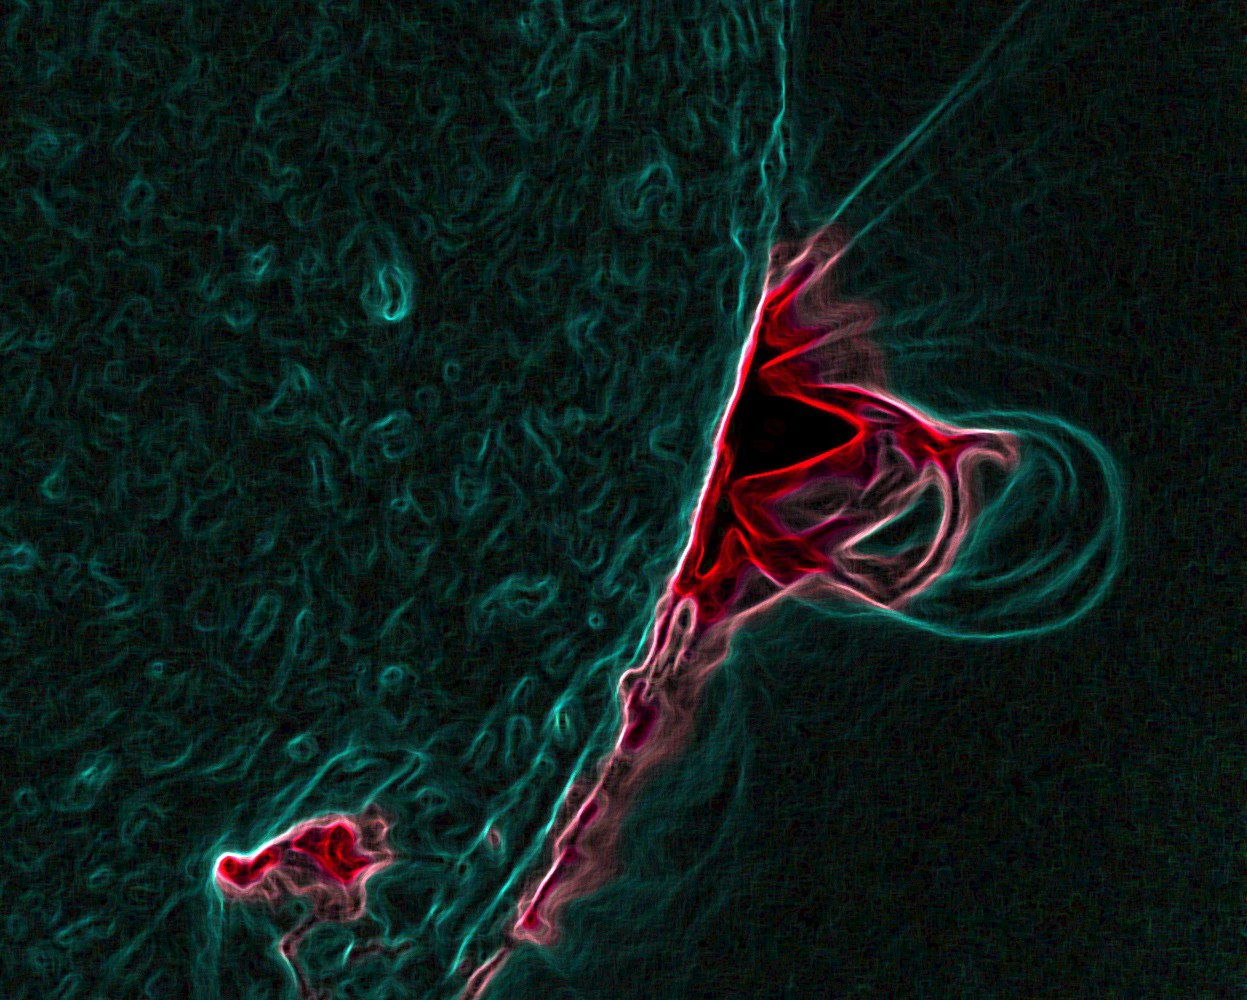
\includegraphics[width=0.72\textwidth]{../figures/t_coronal_loops.jpg}
\caption{太阳表面的磁环：日冕里的等离子体沿着磁通量管发光，管的两个足点扎在光球上。教科书里的"磁面"与"磁通量管"是抽象概念，这张照片是它们在自然界最直白的模样——一根根弯曲的管子，管内热、管外冷，平行与垂直输运的差别就写在明暗对比里。}
\label{fig:photo-appt3}
\figsource{NASA / Goddard Space Flight Center / SDO，CC BY 2.0（Wikimedia Commons）}
\end{figure}

\section{磁通量管上的两条路：平行与垂直输运}
\label{sec:app-t-flux}

要理解磁岛为什么致命，先要看清磁通量管上的"两条路"有多不对称。
平行方向的热输运是电子沿磁力线的自由流动，由 Spitzer 电阻率对应的
电子碰撞时间决定：

\begin{equation}
\tau_e=\frac{3.44\times10^{5}\,T_e^{3/2}}{n_e\ln\Lambda},
\qquad
\ln\Lambda=24-\ln\frac{n_e^{1/2}}{T_e},
\label{eq:app-t-taue}
\end{equation}

式中 $T_e$ 用 eV、$n_e$ 用 $\mathrm{cm^{-3}}$、$\tau_e$ 用 s（NRL 公式，
适用于 $T_e>10\ \mathrm{eV}$）。平行热扩散系数取 Braginskii 的电子热导
（$Z=1$、单位体积除以 $n$ 之后的形式）：

\begin{equation}
\chi_\parallel=\frac{3.16\,T_e\,\tau_e}{m_e},
\label{eq:app-t-chipar}
\end{equation}

$T_e$ 用 J。垂直方向就是附录 S 反推出来的 $\chi_{\mathrm{eff}}$。

\begin{table}[htbp]
  \centering
  \caption{平行与垂直输运的对比。$\chi_\parallel$ 由式 \eqref{eq:app-t-chipar}，
    $\chi_\perp$ 取附录 S 的有效输运系数（两者都是"扩散系数"口径，可直接相比）。
    $\ln\Lambda$ 由式 \eqref{eq:app-t-taue} 给出。}
  \label{tab:app-t-transport}
  \begin{tabular}{@{}p{2.6cm}p{1.3cm}p{1.4cm}p{2.3cm}p{2.2cm}p{1.7cm}p{2.2cm}@{}}
    \toprule
    装置 & $T$ [keV] & $\ln\Lambda$ & $\tau_e$ [s] & $\chi_\parallel$ & $\chi_\perp$ & $\chi_\parallel/\chi_\perp$ \\
    & & & & [$\mathrm{m^2/s}$] & [$\mathrm{m^2/s}$] & \\
    \midrule
    D1 ITER 量级 & $9.194$ & $17.00$ & $1.766\times10^{-4}$ & $9.023\times10^{11}$ & $0.6058$ & $1.490\times10^{12}$ \\
    D2 JET 量级 & $2.336$ & $16.10$ & $6.032\times10^{-5}$ & $7.832\times10^{10}$ & $1.5311$ & $5.115\times10^{10}$ \\
    D3 DIII-D 量级 & $1.649$ & $15.64$ & $2.946\times10^{-5}$ & $2.699\times10^{10}$ & $1.5950$ & $1.692\times10^{10}$ \\
    \bottomrule
  \end{tabular}
\end{table}

表 \ref{tab:app-t-transport} 的最后一列是本附录最重要的数字：
\textbf{平行输运比垂直输运快 $10$ 到 $12$ 个量级}。差距随装置变大而变大，
因为 $\tau_e\propto T^{3/2}/n$，而 D1 的 $T$ 是 D3 的 $5.6$ 倍。

把这两个数放到同一根管子上，感受会更直接。D1 的 $\chi_\parallel=9.02\times10^{11}\ \mathrm{m^2/s}$：

\begin{itemize}
  \item 沿磁力线走完绕环一周的 $L_\parallel=2\pi R=38.96\ \mathrm{m}$：
        $t_\parallel\sim L_\parallel^2/\chi_\parallel=1.68\times10^{-9}\ \mathrm{s}$；
  \item 横越 $1\ \mathrm{cm}$：$t_\perp\sim(0.01)^2/\chi_\perp=1.65\times10^{-4}\ \mathrm{s}$。
\end{itemize}

\textbf{沿磁力线跑 $39\ \mathrm{m}$ 比横着挪 $1\ \mathrm{cm}$ 还快 $5$ 个量级}（比值 $9.8\times10^{4}$）。
这就是"磁通量管"这个词的全部含义：电子在管子里几乎是一维自由气体，而走出管子难如登天。

\begin{tip}{岛内等温：为什么可以"假定温度是平的"}{tip-app-t-flat}
若某个区域被磁场扰动连通成一条长管，温度在该区域的平坦化时间是
$\tau_{\mathrm{flat}}\sim w^2/\chi_\parallel$（$w$ 为区域尺度）。
$w\sim0.07\ \mathrm{m}$、$\chi_\parallel\sim10^{12}\ \mathrm{m^2/s}$ 时
$\tau_{\mathrm{flat}}\sim10^{-14}\ \mathrm{s}$——比能量约束时间小 $15$ 个量级。
\textbf{所以"磁岛内部温度是平的"不是近似，而是硬性结论}；
反过来说，只要出现连通结构，局部温度梯度就一定会被抹平。
\end{tip}

{\footnotesize
\textbf{出处：}Spitzer 电阻率与电子碰撞时间见 NRL《Plasma Formulary》
（2013 修订版，电阻率与碰撞时间两节）；Braginskii 电子热导见
Braginskii（Reviews of Plasma Physics \textbf{1}，205，1965）；
$\chi_\parallel$ 与 $\chi_\perp$ 的量级对比沿用 Wesson《Tokamaks》第 4 版第 14 章。
式 \eqref{eq:app-t-taue}、式 \eqref{eq:app-t-chipar} 与三台装置的全部数值
由仓库脚本按上述公式独立复算。
}

\section{磁岛：共振扰动的几何}
\label{sec:app-t-island}

现在把 T.2 节的共振与 T.3 节的平行输运合起来。设有理面 $q=m/n$ 上存在一个 helical
磁通扰动 $\tilde\Psi\cos\xi$（$\xi=m\theta-n\phi$，$\tilde\Psi$ 单位为 Wb/rad）。
把螺旋磁通 $\Psi_h(r)\equiv\Psi_p(r)-(n/m)\Phi_t(r)$（$\Psi_p$、$\Phi_t$ 为极向与环向磁通）
在有理面附近展开：$\Psi_h'$ 在 $q=m/n$ 处为零（这正是式 \eqref{eq:app-t-resonance}），
而二阶导数等于

\begin{equation}
\Psi_h''(r_{mn})=B_\theta\,s ,
\label{eq:app-t-psih}
\end{equation}

于是分界线条件（$x$ 点与 $o$ 点的螺旋磁通落差为 $2\tilde\Psi$）给出半宽
$x=2\sqrt{\tilde\Psi/(B_\theta s)}$，全宽再乘 $2$。磁力线方程因此给出\textbf{岛}的边界：
它是一族闭合曲线，其中最大的一条叫分界线（separatrix），岛的全宽是

\begin{equation}
w=4\sqrt{\frac{\tilde\Psi}{B_\theta\,s}}
\;=\;4\sqrt{\frac{\tilde\Psi\,q\,R}{B\,r\,s}},
\label{eq:app-t-width}
\end{equation}

第二式用了式 \eqref{eq:app-t-bo}，便于只用环向场 $B$ 估算。\textbf{式
\eqref{eq:app-t-width} 的读法}：$\tilde\Psi$ 是分子，$B_\theta$ 与剪切 $s$ 都在分母——
扰动磁通越大、极向场越弱、剪切越小，岛越宽。系数 $4$ 的来历就是上面两步：
$2$（落差）$\times\,2$（半宽到全宽），中间的开根号把 $\tilde\Psi$ 变成 $\sqrt{\tilde\Psi}$。

\begin{table}[htbp]
  \centering
  \caption{教学扰动 $\tilde\Psi=10^{-4}\ \mathrm{Wb/rad}$ 下三个装置的岛宽（式
    \eqref{eq:app-t-width}）。$\tau_{\mathrm{flat}}=w^2/\chi_\parallel$ 是岛内等温时间，
    $\tau_E$ 取附录 S 的 IPB98(y,2) 值。}
  \label{tab:app-t-w}
  \begin{tabular}{@{}p{3.0cm}p{1.4cm}p{1.6cm}p{1.7cm}p{1.5cm}p{1.6cm}p{1.4cm}p{2.4cm}@{}}
    \toprule
    装置 & $q$ 面 & $r$ [m] & $B_\theta$ [T] & $s$ & $w$ [m] & $w/a$ & $\tau_{\mathrm{flat}}$ [s] \\
    \midrule
    D1 ITER 量级 & $3/2$ & $0.9608$ & $0.5475$ & $0.6000$ & $0.0698$ & $0.0349$ & $5.398\times10^{-15}$ \\
    D1 ITER 量级 & $2/1$ & $1.3960$ & $0.5967$ & $0.9500$ & $0.0531$ & $0.0266$ & $3.128\times10^{-15}$ \\
    D2 JET 量级 & $3/2$ & $0.5190$ & $0.3507$ & $0.6667$ & $0.0827$ & $0.0662$ & $8.738\times10^{-14}$ \\
    D2 JET 量级 & $2/1$ & $0.7340$ & $0.3720$ & $1.0000$ & $0.0656$ & $0.0525$ & $5.492\times10^{-14}$ \\
    D3 DIII-D 量级 & $3/2$ & $0.3044$ & $0.2551$ & $0.8667$ & $0.0851$ & $0.1270$ & $2.681\times10^{-13}$ \\
    D3 DIII-D 量级 & $2/1$ & $0.4048$ & $0.2545$ & $1.1500$ & $0.0739$ & $0.1103$ & $2.025\times10^{-13}$ \\
    \bottomrule
  \end{tabular}
\end{table}

表 \ref{tab:app-t-w} 有两条反直觉的结论，都值得停下来看：

\textbf{（1）同样的扰动磁通，绝对岛宽几乎一样（$5$--$9\ \mathrm{cm}$），但相对尺寸差 $4$ 倍。}
$\tilde\Psi=10^{-4}\ \mathrm{Wb/rad}$ 在 D1 上只占小半径的 $3.5\%$，在 D3 上却占 $12.7\%$。
原因全在式 \eqref{eq:app-t-width} 的分母：$B_\theta\propto B a/(qR)$，大装置的大 $R$
把 $B_\theta$ 抬上去，岛反而被压窄。\textbf{"大装置对磁岛更宽容"是定量的}。

\textbf{（2）$2/1$ 岛比 $3/2$ 岛窄。}D1 上 $w_{2/1}=0.0531\ \mathrm{m}<w_{3/2}=0.0698\ \mathrm{m}$，
虽然 $2/1$ 面的 $r$ 更大（$B_\theta$ 更大、$s$ 也更大，两项都在分母）。
但下一节会看到：$2/1$ 岛的\textbf{位置}比宽度更麻烦。

$2/1$ 面的 $\tau_{\mathrm{flat}}=w^2/\chi_\parallel=3.128\times10^{-15}\ \mathrm{s}$
同样远小于 $\tau_E=2.476\ \mathrm{s}$。岛内温度被抹平这一条，对两个面都成立。

{\footnotesize
\textbf{出处：}岛宽公式的标准推导见 Wesson《Tokamaks》第 4 版第 3 章与第 6 章
（磁岛与撕裂模）；Fitzpatrick《Plasma Physics: An Introduction》第 9 章给出同一结果的
教学推导；螺旋磁通与分界线的几何见 Hazeltine \& Meiss《Plasma Confinement》第 6 章。
本节的数值口径（$\tilde\Psi=10^{-4}\ \mathrm{Wb/rad}$ 作为教学扰动）自拟，
全部数字由仓库脚本复算。
}

\section{岛链重叠、随机化与约束崩塌}
\label{sec:app-t-overlap}

一个岛只是把一层磁面撕开；一排\textbf{岛链}（$m/n=3/2$、$2/1$、$3/1$……）叠在一起时，
相邻有理面之间的"好磁面"会被两侧的岛吃掉。用 Chirikov 量级判据：当两个岛链的
半宽之和超过它们所在有理面的间距时，磁力线开始\textbf{随机行走}：

\begin{equation}
\frac{w_1}{2}+\frac{w_2}{2}\;\gtrsim\;\Delta r
\qquad\Longleftrightarrow\qquad
\tilde\Psi\;\gtrsim\;B_\theta s\left(\frac{\Delta r}{4}\right)^2 .
\label{eq:app-t-overlap}
\end{equation}

\begin{table}[htbp]
  \centering
  \caption{$3/2$ 与 $2/1$ 岛链重叠所需的扰动磁通（式 \eqref{eq:app-t-overlap}）。
    最后一列是相对教学值 $\tilde\Psi=10^{-4}\ \mathrm{Wb/rad}$ 的倍数。}
  \label{tab:app-t-overlap}
  \begin{tabular}{@{}p{3.0cm}p{1.7cm}p{1.7cm}p{1.6cm}p{2.8cm}p{2.0cm}@{}}
    \toprule
    装置 & $r_{3/2}$ [m] & $r_{2/1}$ [m] & $\Delta r$ [m] & $\tilde\Psi_{\text{重叠}}$ [Wb/rad] & 相对教学值 \\
    \midrule
    D1 ITER 量级 & $0.9608$ & $1.3960$ & $0.4352$ & $6.710\times10^{-3}$ & $67.1$ 倍 \\
    D2 JET 量级 & $0.5190$ & $0.7340$ & $0.2150$ & $1.075\times10^{-3}$ & $10.7$ 倍 \\
    D3 DIII-D 量级 & $0.3044$ & $0.4048$ & $0.1005$ & $1.847\times10^{-4}$ & $1.8$ 倍 \\
    \bottomrule
  \end{tabular}
\end{table}

表 \ref{tab:app-t-overlap} 是一张\textbf{安全裕度表}：

\textbf{（1）装置的"抗岛能力"随尺寸急剧上升。}D3 只需要 $1.8$ 倍教学扰动就能让岛链重叠，
D1 需要 $67$ 倍。原因有两层：$\Delta r$ 随 $a$ 变大，而 $\tilde\Psi\propto(\Delta r)^2$；
同时 $B_\theta s$ 也在变大。\textbf{小装置更容易被"小岛"毁掉}，
这也解释了为什么破裂物理在小装置上更容易做实验。

\textbf{（2）随机化不是"更差的输运"，而是"另一类输运"。}磁力线一旦随机行走，
电子沿磁力线的自由程被截断成"随机步长"$\Delta r$，输运从回旋玻姆量级跳到
\textbf{玻姆甚至更差}（附录 S S.3 节已经算过两者差两个量级）。
这正是历史上"玻姆扩散支配的年代"里装置放大无效的物理原因。

\textbf{（3）判据是量级判据，不是开关。}式 \eqref{eq:app-t-overlap} 忽略了岛宽的
互相修正、磁力线的实际缠绕与等离子体流对岛的屏蔽；工程上更常用的是
"岛宽与 $\Delta r$ 同量级就要警惕"。本表的作用是给出\textbf{量级和标度}，
不用于判定某台装置的运行边界。

{\footnotesize
\textbf{出处：}岛链重叠与随机磁场见 Chirikov（Physics Reports \textbf{52}，263，1979）
的共振重叠判据；托卡马克上的应用见 Wesson《Tokamaks》第 4 版第 3 章
（随机磁场与输运）；Hazeltine \& Meiss《Plasma Confinement》第 6、10 章。
本表的三行数值由仓库脚本按式 \eqref{eq:app-t-overlap} 复算。
}

\section{新经典撕裂模与 $\beta$ 极限}
\label{sec:app-t-ntm}

磁岛一旦出现，会不会自己长大？这取决于撕开的能量账。经典撕裂模由电流剖面的
自由能驱动，判据写成 $\Delta'$（有理面两侧磁通扰动的对数导数跳变）。真实装置里
还有一项：\textbf{自举电流}（bootstrap current，由压强梯度在环形位形中自然产生，
附录 M 已介绍）会在岛内被抹平，形成附加驱动。把两项放进 Rutherford 方程：

\begin{equation}
\frac{\mu_0}{1.22\eta}\frac{\diff w}{\diff t}
=\Delta'(w)+\underbrace{5.6\,\frac{\mu_0 j_{\mathrm{bs}}L_q}{B_\theta\,w}}_{\Delta'_{\mathrm{bs}}(w)} ,
\qquad
L_q\equiv\frac{q}{q'},
\label{eq:app-t-rutherford}
\end{equation}

其中 $\eta$ 是电阻率，$j_{\mathrm{bs}}$ 是自举电流密度。$\Delta'_{\mathrm{bs}}\propto1/w$：
$w$ 小时它很大，$w$ 大时被稀释。令它与经典项 $|\Delta'_0|$ 相等，得到\textbf{临界岛宽}

\begin{equation}
w_{\mathrm{marg}}=\frac{5.6\,\mu_0\,j_{\mathrm{bs}}\,L_q}{B_\theta\,|\Delta'_0|},
\label{eq:app-t-wmarg}
\end{equation}

小于它的种子岛会被电阻扩散抹掉，大于它的会一路长到饱和——这就是
\textbf{新经典撕裂模（NTM）}。它不由外部误差场驱动，而是由等离子体自己的自举电流驱动，
所以不能靠"把磁场做干净"解决。

\begin{table}[htbp]
  \centering
  \caption{$2/1$ 面的 NTM 临界岛宽（式 \eqref{eq:app-t-wmarg}）。教学取值：
    自举电流份额 $f_{\mathrm{bs}}=j_{\mathrm{bs}}/j_\phi=0.25$；
    $|\Delta'_0|$ 取 $20$、$50$、$100\ \mathrm{m^{-1}}$ 做敏感性表。
    $j_\phi=I_p/(\pi a^2\kappa)$。}
  \label{tab:app-t-ntm}
  \begin{tabular}{@{}p{2.6cm}p{2.0cm}p{2.0cm}p{1.0cm}p{1.3cm}p{2.2cm}p{1.4cm}p{1.4cm}@{}}
    \toprule
    装置 & $j_\phi$ [A/m$^2$] & $j_{\mathrm{bs}}$ [A/m$^2$] & $L_q$ [m] & $B_\theta$ [T] & $w_{\mathrm{marg}}$ & $w_{\mathrm{marg}}$ & $w_{\mathrm{marg}}$ \\
    & & & & & $|\Delta'_0|=20$ & $=50$ & $=100$ \\
    \midrule
    D1 ITER 量级 & $7.022\times10^{5}$ & $1.755\times10^{5}$ & $1.469$ & $0.5967$ & $15.21\ \mathrm{cm}$ & $6.08\ \mathrm{cm}$ & $3.04\ \mathrm{cm}$ \\
    D2 JET 量级 & $4.365\times10^{5}$ & $1.091\times10^{5}$ & $0.734$ & $0.3720$ & $7.58\ \mathrm{cm}$ & $3.03\ \mathrm{cm}$ & $1.52\ \mathrm{cm}$ \\
    D3 DIII-D 量级 & $5.909\times10^{5}$ & $1.477\times10^{5}$ & $0.352$ & $0.2545$ & $7.19\ \mathrm{cm}$ & $2.88\ \mathrm{cm}$ & $1.44\ \mathrm{cm}$ \\
    \bottomrule
  \end{tabular}
\end{table}

表 \ref{tab:app-t-ntm} 的读法与"答案"这个词无关，它给的是\textbf{标度与量级}：

\textbf{（1）临界岛宽是厘米级。}三台装置在 $|\Delta'_0|=50\ \mathrm{m^{-1}}$ 时都给出
$3$--$6\ \mathrm{cm}$，换算成相对尺寸是 $w/a=0.030$（D1）到 $0.043$（D3）。
也就是说，\textbf{一个百分之几小半径的种子岛就足以启动 NTM}——
这与 T.4 节的教学岛宽（$0.027$--$0.127$）正好接上：教学扰动给出的岛已经在临界值附近。

\textbf{（2）装置越大，绝对临界岛宽越大，但相对值越小。}D1 的 $w_{\mathrm{marg}}/a=0.030$，
D3 是 $0.043$：大装置对 NTM 的相对裕度更大，但绝对尺寸要求更严（$6\ \mathrm{cm}$ 的
种子岛在 $2\ \mathrm{m}$ 半径上不算小）。

\textbf{（3）$|\Delta'_0|$ 的不确定性是 $5$ 倍，结果差 $5$ 倍。}表中三列相差 $5$ 倍，
不是计算误差，而是\textbf{电流剖面未知}带来的真实不确定性。所以工程上用 NTM 判据时
从不只看一个数，而是做参数扫描。真实装置还依赖\textbf{等离子体旋转对岛的屏蔽}
（旋转使扰动在岛的参考系里带频率，被电阻层屏蔽），一旦旋转被刹车，NTM 就长起来——
这是"旋转是资产"的最硬理由。

{\footnotesize
\textbf{出处：}修正 Rutherford 方程与 NTM 综述见 La Haye（Physics of Plasmas
\textbf{13}，055501，2006）；自举电流的推导见 Wesson《Tokamaks》第 4 版第 4 章；
$\beta_N$ 与密度极限等运行极限见附录 M 的 M.5 节（$\beta_N$ 定义、$n_G$ 与 H 模阈值）。
$f_{\mathrm{bs}}=0.25$ 与 $|\Delta'_0|$ 的取值是教学假设，表中数值由仓库脚本复算。
}

\section{锯齿、内部输运垒与剖面刚度}
\label{sec:app-t-sawtooth}

拓扑的另一个后果在轴心。$q_0<1$ 时轴心附近存在 $q=1$ 面，$m/n=1/1$ 的内扭曲模
在那里不稳定，会周期性地把芯部"翻出去"再重建——这就是\textbf{锯齿}
（sawtooth）。用式 \eqref{eq:app-t-qprofile} 直接读出反转半径：

\begin{equation}
r_{\mathrm{inv}}=a\sqrt{\frac{1-q_0}{q_{95}-q_0}}
\qquad(q_0<1),
\label{eq:app-t-rinv}
\end{equation}

$q_0\ge1$ 时该式无解，\textbf{轴心不存在 $q=1$ 面，也就不出现 $1/1$ 锯齿}。
表 \ref{tab:app-t-surfaces} 已经给出三台装置的位置：D1（$q_0=1.05$）与
D2（$q_0=1.00$）都没有 $q=1$ 面；\textbf{只有 D3（$q_0=0.85$）有}，
$r_{\mathrm{inv}}=0.1462\ \mathrm{m}$，即 $\rho=0.218$，混合区占横截面份额
$\rho^2=4.8\%$。

\textbf{两个推论。}

\textbf{（1）"有没有锯齿"由 $q_0$ 与 $1$ 的大小关系决定，而不是由装置大小决定。}
D3 比 D1 小得多，却是唯一有锯齿的一台。反过来说，把 $q_0$ 抬到 $1$ 以上
（靠电流剖面展平，例如低杂波电流驱动或电子回旋加热）就能压掉锯齿——
代价是轴心电流梯度被展平，可能诱发其他不稳定性。

\textbf{（2）锯齿与内部输运垒（ITB）是一对反例。}锯齿是"轴心梯度被周期性抹平"，
ITB 是"某处梯度突然变陡且稳定存在"。后者出现在 $q$ 剖面的极值面（$q'=0$，
即 $s=0$ 处）：剪切为零的地方，湍流被抑制，输运下降，梯度堆起来。
式 \eqref{eq:app-t-shear} 里令 $q'=0$ 就得到 $s=0$ 的位置，读者可用表
\ref{tab:app-t-surfaces} 的 $q'$ 列判断教学剖面是否给出 $s=0$（本教学剖面单调，
故 $s>0$ 处处成立，\textbf{不含 ITB}——这是教学剖面刻意简化的地方）。

\textbf{（3）与附录 S 的外推问题接上。}附录 S S.9 节说他输运不能按玻姆外推；
本附录补上原因：\textbf{只要磁拓扑保持完整，输运就停在回旋玻姆量级；
一旦拓扑被破坏（岛链重叠、随机化），输运跳到玻姆或更差}。所以"能不能外推"
这个问题的一半答案在拓扑上：外推的合法性依赖于\textbf{新装置里磁面是否还是好的}。

{\footnotesize
\textbf{出处：}锯齿与 $m/n=1/1$ 内扭曲模见 Wesson《Tokamaks》第 4 版第 3 章；
ITB 与剪切抑制湍流见 Connor 等（Nuclear Fusion \textbf{44}，R1，2004）的综述；
剖面刚度与临界梯度见附录 S S.9 节引用的同一批文献。$r_{\mathrm{inv}}$ 由式
\eqref{eq:app-t-rinv} 直接计算。
}

\section{六道估算练习}
\label{sec:app-t-problems}

这六道题按 T.1 到 T.7 的顺序排，答案都可以用仓库脚本 \texttt{tools/\allowbreak{}calc/\allowbreak{}appT\_calc.py} 复算。

\textbf{练习 1（有理面位置）}。D1 量级取 $q_0=1.05$、$q_{95}=3.00$、$a=2.00\ \mathrm{m}$，
用式 \eqref{eq:app-t-qprofile} 求 $q=3/2$ 面的 $\rho$ 与 $r$。

\textbf{解答}：$\rho=\sqrt{(1.5-1.05)/(3.00-1.05)}=\sqrt{0.45/1.95}=0.4804$，
$r=\rho a=0.9608\ \mathrm{m}$。注意 $q=2$ 面在 $r=1.3960\ \mathrm{m}$ 处，
两个面之间只有 $0.4352\ \mathrm{m}$——这正是 T.5 节岛链重叠的分母。

\textbf{练习 2（局部量与剪切）}。对上题的有理面，求 $B_\theta$、$q'$ 与 $s$。

\textbf{解答}：由式 \eqref{eq:app-t-shear}，$q'=2(3.00-1.05)\times0.9608/2.00^2=0.9367\ \mathrm{m^{-1}}$；
$s=rq'/q=0.9608\times0.9367/1.5=0.6000$。
由式 \eqref{eq:app-t-bo}，$B_\theta=5.3\times0.9608/(1.5\times6.20)=0.5475\ \mathrm{T}$，
即 $B_\theta/B=0.5475/5.3=0.1033$——只有环向场的 $10.3\%$。

\textbf{练习 3（岛宽对标度）}。其他条件不变，把扰动磁通从 $10^{-4}$ 增到
$4\times10^{-4}\ \mathrm{Wb/rad}$，D1 的 $3/2$ 岛宽变成多少？是原来的几倍？

\textbf{解答}：$w=4\sqrt{\tilde\Psi/(B_\theta s)}$，故 $w\propto\sqrt{\tilde\Psi}$：
$w=0.0698\times\sqrt4=0.1396\ \mathrm{m}$，是原来的 $2.00$ 倍。
\textbf{磁通要涨 $4$ 倍，岛宽才涨 $2$ 倍}——这是"误差场容差"这类工程指标里的开方式。

\textbf{练习 4（岛内等温时间）}。D1 的 $\chi_\parallel=9.023\times10^{11}\ \mathrm{m^2/s}$、
$w=0.0698\ \mathrm{m}$、$\tau_E=2.4762\ \mathrm{s}$，求 $\tau_{\mathrm{flat}}$ 并比较。

\textbf{解答}：$\tau_{\mathrm{flat}}=w^2/\chi_\parallel=5.398\times10^{-15}\ \mathrm{s}$，
比 $\tau_E$ 小 $15$ 个量级（比值 $2.18\times10^{-15}$）。
所以"岛内温度是平的"是硬结论：岛内不可能维持梯度。

\textbf{练习 5（岛链重叠）}。D1 的 $3/2$ 与 $2/1$ 面间距 $\Delta r=0.4352\ \mathrm{m}$，
$2/1$ 面 $B_\theta=0.5967\ \mathrm{T}$、$s=0.9500$。求让两条岛链重叠所需的 $\tilde\Psi$。

\textbf{解答}：由式 \eqref{eq:app-t-overlap}，
$\tilde\Psi\gtrsim B_\theta s(\Delta r/4)^2=0.5967\times0.9500\times(0.1088)^2
=6.710\times10^{-3}\ \mathrm{Wb/rad}$，是教学值的 $67.1$ 倍。
\textbf{大装置的抗岛裕度是"平方级"的}：间距 $0.435\ \mathrm{m}$ 对应 $6.7\ \mathrm{mWb/rad}$。

\textbf{练习 6（锯齿反转半径）}。D3 量级取 $q_0=0.85$、$q_{95}=4.00$、$a=0.67\ \mathrm{m}$，
求反转半径与混合区体积份额。D1（$q_0=1.05$）呢？

\textbf{解答}：D3 由式 \eqref{eq:app-t-rinv}，
$r_{\mathrm{inv}}=0.67\sqrt{0.15/3.15}=0.1462\ \mathrm{m}$（$\rho=0.2182$），
混合区体积份额 $\rho^2=4.8\%$。D1 的 $q_0=1.05>1$，式 \eqref{eq:app-t-rinv} 无解：
\textbf{轴心没有 $q=1$ 面，不出现 $1/1$ 锯齿}。

\section{来源、分级与版权说明}
\label{sec:app-t-source}

\begingroup\small
\begin{table}[htbp]
  \centering
  \caption{附录 T 各节的借鉴来源与独立性说明（与配套手册 J 的逐章对照表、附录 S 的来源表 
ef{tab:app-s-source} 同一体例）。}
  \label{tab:app-t-source}
  \begin{tabular}{@{}p{1.1cm}p{4.4cm}p{3.4cm}p{6.4cm}@{}}
    \toprule
    节 & 借鉴来源 & 借鉴内容 & 本书的处理 \\
    \midrule
    T.1 & Wesson《Tokamaks》；Chen《Introduction to Plasma Physics》 & 磁面、磁通函数、$q$ 的定义 & 表 \ref{tab:app-t-q95} 的 $q_0$、$q_{95}$ 与差值自拟 \\
    T.2 & Wesson 第 3 章；Fitzpatrick 第 9 章 & 有理面与 $k_\parallel$ 的共振条件 & 教学剖面式 \eqref{eq:app-t-qprofile} 与两表数值自算 \\
    T.3 & NRL《Plasma Formulary》；Braginskii 1965 & 电子碰撞时间与平行热导公式 & 三台装置的 $\chi_\parallel/\chi_\perp$ 与时间对比自算 \\
    T.4 & Wesson 第 3、6 章 & 岛宽公式与分界线几何 & 教学扰动 $\tilde\Psi=10^{-4}$ 自拟，岛宽表自算 \\
    T.5 & Chirikov 1979；Hazeltine \& Meiss & 共振重叠判据 & 重叠阈值表与"平方级裕度"结论自算 \\
    T.6 & La Haye 2006；Wesson 第 4 章 & 修正 Rutherford 方程与 NTM & $f_{\mathrm{bs}}$、$|\Delta'_0|$ 作教学假设，敏感性表自算 \\
    T.7 & Wesson 第 3 章；Connor 等 2004 & 锯齿、ITB 与剪切抑制 & $r_{\mathrm{inv}}$ 与"教学剖面不含 ITB"的说明自拟 \\
    \bottomrule
  \end{tabular}
\end{table}

\textbf{不复制声明}（与附录 I、S 同一口径）：

\begin{enumerate}
  \item \textbf{不复制图。}本附录没有引用任何文献的图；所有结论以公式与数字表达，
        需要图的读者请回原书（Wesson 第 3 章有磁面与岛链的经典插图）。
  \item \textbf{不复制表。}表 \ref{tab:app-t-q95} 到表 \ref{tab:app-t-ntm} 的数值
        全部由仓库脚本 \texttt{tools/\allowbreak{}calc/\allowbreak{}appT\_calc.py} 从公式复算，不是从文献表中转录。
  \item \textbf{不复制文字。}公式是公共知识（标准结果），但\textbf{解释、例题、口径与
        取舍是本书自己的}；每题答案都写了"这个数字从哪里来"。
  \item \textbf{不给 DOI。}参考文献只给书名、作者、年份与卷期；
        需要精确引用的读者请以最新版原书为准。
\end{enumerate}

\textbf{分级建议}：T.1--T.3 属于"读完第 5、8 章后即可读"；T.4--T.6 需要第 9 章
（不稳定性）作为背景；T.7 与附录 S 配合读效果最好。全部内容属于\textbf{专题级}，
不进入正文主线，也不作为任何考试范围的隐含要求。

\textbf{与本书其他部分的接口}：第 5 章（磁流体力学）给出磁面与重联的语言；
第 9 章（不稳定性）给出撕裂模与扭曲模的线性理论；附录 M 给出 $\beta_N$、
$n_G$ 与自举电流；附录 N 给出 ELM 与偏滤器热负荷；附录 S 给出 $\tau_E$、
$\chi_{\mathrm{eff}}$ 与回旋玻姆标度；\textbf{本附录补上它们之间缺的一环——
"磁面什么时候不再是磁面"}。
\endgroup
